% !TEX root = ../popl-paper.tex

In the previous section, we defined several communication models
as classes of MSCs. 
In this section, we provide alternative definitions these 
communication models
fitting closer to the way these communication models are defined in other works. We establish the equivalence
of the two alternative definitions for each concerned model. We also recall the notion of
execution and Chevrou~\emph{et al.} sequential hierarchy of communication models seen as set of
executions.


%\paragraph{\bf Queuing networks}
We consider networks of processes formed by a bunch of FIFO queues that store the messages in transit.
Formally, a \emph{queuing network} is a tuple $\anetwork=(\setofqueuidentifiers,\queuidofprocs)$ such that
$\setofqueuidentifiers$ is a finite set of queue identifiers, and
$\queuidofprocs:\procSet\times\procSet\to \setofqueuidentifiers$ assigns a queue to each
pair of processes.
A queuing network $(\setofqueuidentifiers,\queuidofprocs)$ is $\pp$ if
$\setofqueuidentifiers=\procSet\times\procSet$ and $\queuidofprocs$ is the identity.
The queuing network $(\setofqueuidentifiers,\queuidofprocs)$ is $\mb$ if
$\setofqueuidentifiers=\procSet$ and $\queuidofprocs(p,q)=q$; it is called $\onensymb$ if
$\setofqueuidentifiers=\procSet$ and $\queuidofprocs(p,q)=p$. Finally, it is called
$\nnsymb$ if $\setofqueuidentifiers=\{0\}$ and $\queuidofprocs(p,q)=0$ for all $p,q\in\procSet$.

\paragraph{\bf Configurations, executions, and operational semantics}
A \emph{configuration} of the queuing network $(\setofqueuidentifiers,\queuidofprocs)$ is
a tuple $\aconf=(w_{\aqueueid})_{\aqueueid\in\setofqueuidentifiers}\in (\paylodSet^*)^{\setofqueuidentifiers}$,
where for each queue identifier $\aqueueid$, the queue content $w_{\aqueueid}$ is a finite sequence of messages.
The \emph{initial configuration} $\initconf$ is the one in which all queues are empty, i.e.
$w_{\aqueueid}=\epsilon$ for all $\aqueueid\in\setofqueuidentifiers$.
A \emph{step} is a tuple $(\aconf,a,\aconf')$, (later written $\aconf\actionstep{a}\aconf'$)
where $\aconf=(w_{\aqueueid})_{\aqueueid\in\setofqueuidentifiers}$,
$\aconf'=(w_{\aqueueid}')_{\aqueueid\in\setofqueuidentifiers}$,
$a$ is an action, and the following holds:
\begin{itemize}
  \item if $a=\sact{p}{q}{\msg}$, then $b'_{\aqueueid}=b_{\aqueueid}\cdot \msg$
  and $b_j'=b_j$ for all $j\in \setofqueuidentifiers\setminus\{\aqueueid\}$,
  where $\aqueueid=\queuidofprocs(p,q)$.
  \item if $a=\ract{p}{q}{\msg}$, then $b_{\aqueueid}=\msg\cdot b'_{\aqueueid}$
  and $b_j'=b_j$ for all $j\in \setofqueuidentifiers\setminus\{\aqueueid\}$,
  where $\aqueueid=\queuidofprocs(p,q)$.
\end{itemize}
An \emph{execution} of the queuing network $(\setofqueuidentifiers,\queuidofprocs)$
is a finite sequence of actions $e=a_1a_2\ldots a_n$ such that
$\initconf\actionstep{a_1}\actionstep{a_2}\ldots\actionstep{a_n}\aconf$ for some configuration $\aconf$.
The execution is $\pp$ (resp. $\mb$, $\onensymb$, $\nnsymb$) if its queuing network is.

\begin{example}
The execution
$$
\sact{p}{q}{m_1}\cdot\sact{q}{r}{m_2}\cdot\ract{q}{r}{m_2}\cdot\ract{p}{q}{m_1}
$$
is $\pp$, $\mb$, and $\onensymb$, but it is not $\nnsymb$ (because $m_2$ is received before $m_1$).
\end{example}

\begin{example}
    The execution
    $$
    \sact{p}{q}{m_1}\cdot\sact{r}{q}{m_2}\cdot\ract{r}{q}{m_2}
    $$
    is $\pp$ and $\onensymb$, but it is neither $\mb$ nor $\nnsymb$ (because $m_2$ "overtakes" $m_1$). Note that in the
    final configuration $m_1$ is still in the queue ($m_1$ is "unmatched").
\end{example}


Consider a network $\anetwork$ with two queue identifiers $\aqueueid_1$ and $\aqueueid_2$,
and let $\anetwork'$ be the network obtained by merging the two queues $\aqueueid_1$ and $\aqueueid_2$ in a
same queue. Then $\anetwork'$ imposes more constraints than $\anetwork$ on the sequence of actions it admits,
and any $\anetwork'$-execution also is an $\anetwork$-execution. From this observation, it follows that
the communication models we considered define the hierarchy of executions depicted in
Fig.~\ref{fig:hierarchy-of-executions}. We refer
to~\cite{DBLP:journals/fac/ChevrouHQ16}
for clarifying how the asynchronous, $\rsc$, and $\co$ communication models may
also be defined as sets of executions and fit in this hierarchy; we also refer
to~\cite{DBLP:journals/fac/ChevrouHQ16} for examples illustrating
the strictness of this hierarchy.

\begin{figure}
  \centering
    % !TEX root = ../popl-paper.tex

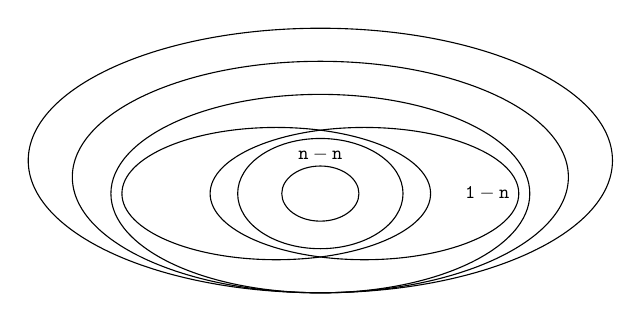
\begin{tikzpicture}[scale=0.7, every node/.style={transform shape}]
   % \draw (0,0) ellipse (5cm and 3cm);
    %\draw (0,0) ellipse (5cm and 3cm);
    %\draw (0,0) ellipse (5cm and 3cm);

\draw(0,0) ellipse (.7cm and .5cm); 
\node (r) at (0,0) {$\rsc$}; 
\draw(0,0) ellipse (1.5cm and 1cm); 
\node (nn) at (0,.7) {$\mathtt{n-n}$}; 

\draw(.8,0) ellipse (2.8cm and 1.2cm); 
\node[left] (n1) at (3.55,0) {$\mathtt{1-n}$}; 
\draw(-.8,0) ellipse (2.8cm and 1.2cm); 
\node[right] (1n) at (-3.5,0) {$\none$}; 

\draw(0,0) ellipse (3.8cm and 1.8cm); 
\node (nn) at (0,1.5) {$\co$}; 

\draw(0,.3) ellipse (4.5cm and 2.1cm); 
\node (nn) at (0,2) {$\oneone$}; 

\draw(0,.6) ellipse (5.3cm and 2.4cm); 
\node (nn) at (0,2.6) {$\asy$}; 

\end{tikzpicture} 

% \begin{tikzpicture}[inclusion/.style={right hook->, thick}]
%     \node (RSC)    at (-1.7,0) {\begin{tabular}{c}synchronous \\ (RSC)\end{tabular}};
%     \node (FIFOnn) at (1,0)  {\begin{tabular}{c}FIFO \\ n-n\end{tabular}}; 
%     \node (FIFO1n) at (3.2,1.5)  {\begin{tabular}{c}FIFO 1-n\end{tabular}};
%     \node (mb)     at (3.2,-1.5) {\begin{tabular}{c}FIFO n-1\\ (mailbox)\end{tabular}};
%     \node (co)     at (5.8,0)  {\begin{tabular}{c}causally\\ ordered\end{tabular}};
%     \node (p2p)    at (8,0) {\begin{tabular}{c}FIFO 1-1\\ (p2p)\end{tabular}};
%     \node (async)  at (10.4,0) {\begin{tabular}{c}asyn-\\ chronous\end{tabular}};
%     \draw[inclusion] (RSC) to (FIFOnn);
%     \draw[inclusion] (FIFOnn.north east) to (FIFO1n.west);
%     \draw[inclusion] (FIFOnn.south east) to (mb.west);
%     \draw[inclusion] (FIFO1n.east) to (co.north west);
%     \draw[inclusion] (mb.east) to (co.south west);
%     \draw[inclusion] (co) to (p2p);
%     \draw[inclusion] (p2p) to (async);
% \end{tikzpicture}
    \caption{\label{fig:hierarchy-of-executions} Hierarchy of communication models based on  sets of
    executions (taken from~\cite{DBLP:journals/fac/ChevrouHQ16})}
\end{figure}

To conclude this brief discussion on queuing networks and executions, we clarify in what sense the operational semantics we introduced in this section are sound and complete with respect to the axiomatic definitions of the communication models we gave in Section~\ref{sec:MSC}. Remember that a linearization $\linrel$ of a MSC
defines a total order on its events, and therefore an execution.

\begin{fact}
A MSC $\msc$ is $\pp$ (resp. $\mb$, $\onensymb$, $\nnsymb$) if and only if there exists
a linearization $\linrel$ of $\msc$ that induces a $\pp$ execution (resp. a $\mb$, $\onensymb$, $\nnsymb$ execution).
\end{fact}

Note that, moreover, a MSC $\msc$ is $\pp$ if and only if \emph{all} of its linearizations induce $\pp$ executions.